\chapter{Introduzione}\label{ch:introduzione}
Negli ultimi due anni, a causa della crisi pandemica, abbiamo assistito ad un aumento 
esponenziale del commercio online:
secondo ISTAT nel nostro paese si è registrato un aumento del 50,2\% nelle vendite 
e-commerce.\cite{istat}
Il lavoro inoltre ha subito un cambiamento repentino, facendo migrare milioni di persone
 dall'ufficio alle loro mura domestiche.
Tutti questi fenomeni si sono realizzati grazie a internet, che ha accolto tutte quelle
 interazioni che fino a qualche mese prima
erano fatte fisicamente.
Questo ha portato ad avere sempre più traffico e una maggiore richiesta di robustezza, 
sicurezza e ridondanza da parte delle aziende.
Basti pensare al danno economico che hanno 
avuto le oltre \textbf{200 milioni} di attività commerciali che stavano pubblicizzando i 
loro beni su Facebook durante
le 14 ore di disservizi lo scorso 4 ottobre\cite{fbdown}.
\\\\
Organizzare il lavoro per lo sviluppo di applicazioni web di grandi dimensioni, capaci di 
accogliere numeri sempre maggiori di utenti, non è per niente banale, ed è molto interessante
capire come suddividere le responsabilità tra i vari team che contribuiscono alla sua realizzazione
 e mantenimento.
\\
L'approccio più diffuso per affrontare il problema è quello di suddividere le persone per 
competenze (ovvero in modo \emph{orizzontale}), creando team che mettano in comune
figure con abilità dello stesso ambito. Il classico approccio monolitico infatti prevede due
 suddivisioni, la parte \emph{frontend}, che si occupa dell'esperienza 
utente e la parte \emph{backend}, che invece gestisce server, basi di dati e servizi. 
\\\\
Quando però il progetto aumenta di complessità, si sente la necessità 
di suddividere il lavoro in sotto-progetti, e l'approccio orizzontale potrebbe non essere la scelta
 migliore, in quanto potrebbe rallentare l'introduzione di nuove funzionalità.
\\
Nello sviluppo della parte backend, si è risolto il problema vedendo l'intero blocco come un
insieme di \textbf{microservizi} autonomi di piccole dimensioni che comunicano tra loro tramite API ben definite.
\begin{figure}[H]
    \centering
    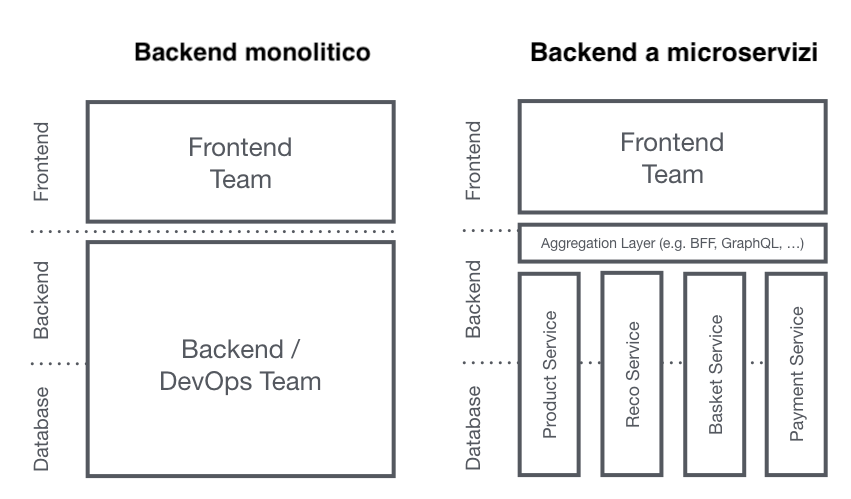
\includegraphics[width=140mm]{img/monolite}
    \caption{Lo schema rappresenta il blocco unico dalla parte frontend, e invece la suddivizione per 
    microservizi attuata nella parte backend}
  \end{figure}
Analogamente, nel mondo frontend, si è superato l'approccio monolitico, imitando quello che già è 
successo per la parte backend.
\\
Possiamo allora pensare di formare in maniera diversa i team di sviluppo: pensare di avere in un unico gruppo
le figure necessarie per affrontare a 360 gradi un sottoprogetto, con differenti competenze al
loro interno, per fargli seguire un obiettivo comune. L'obiettivo è creare team accomunati da una missione, e non da certe competenze.
\begin{figure}[H]
    \centering
    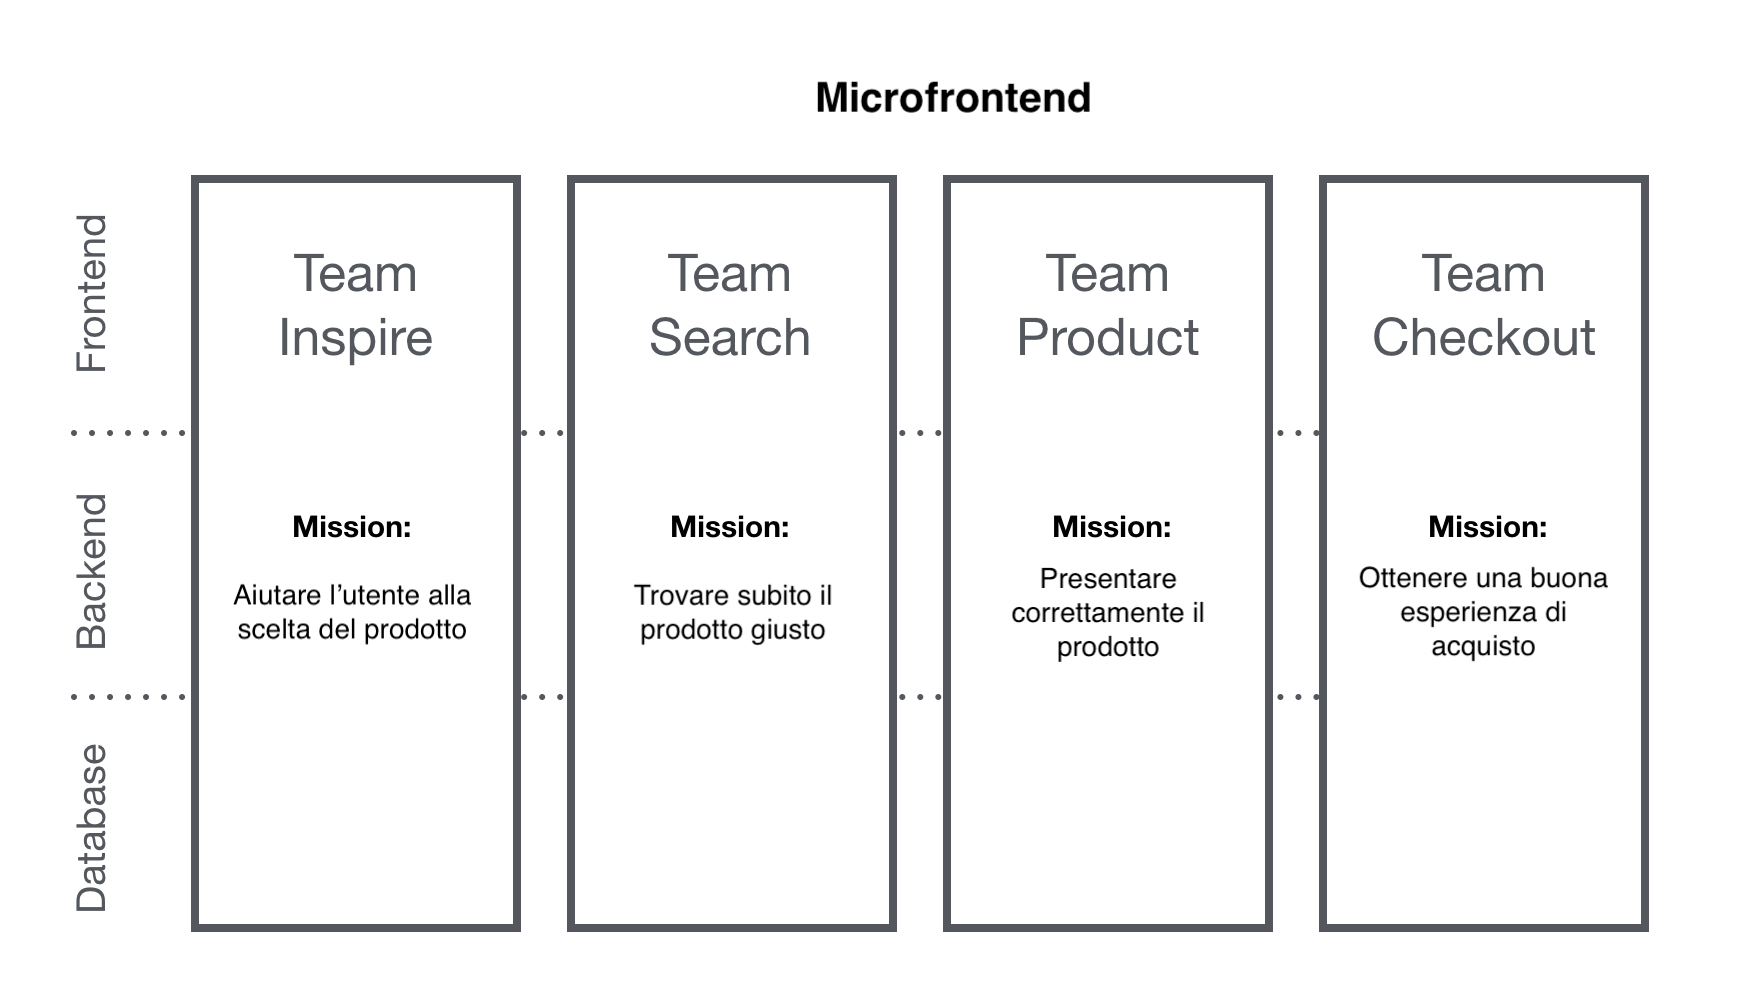
\includegraphics[width=140mm]{img/microfrontend}
    \caption{Grazie all'architettura microfrontend, ogni team, guidato da un obiettivo, gestisce una 
    parte del progetto nella sua interezza}
  \end{figure}
  Di seguito vedremo da vicino le metodologie utilizzate per realizzare un'architettura microfrontend:
partendo dalla definizione e realizzazione di un microfrontend, la composizione di questi in un'unica pagina e le varie tecnologie
  a disposizione, discutendo pregi e difetti di ognuna.
  Ci soffermeremo inoltre sui sistemi di comunicazione adottati, per far dialogare i vari componenti del progetto, e come organizzare 
  la creazione di un design system uniforme.
\\\\
  Successivamente introdurremo il progetto realizzato durante il tirocinio con l'azienda Leonardo SPA: l'applicazione dell'approccio microfrontend
  al progetto di un'innovativa applicazione web per la gestione di sale di comando e controllo.

